\section{Primeiro objetivo - probabilidades}

No primeiro objetivo iremos comparar os resultados de várias probabilidades
obtidas através do modelo desenvolvido com os de uma simulação.
Iremos observar 5 cenários, alterando a janela de contenção máxima (\textit{m}):

\begin{itemize}
    \item \textit{m} = 0;
    \item \textit{m} = 1;
    \item \textit{m} = 4;
    \item \textit{m} = 8;
    \item \textit{m} = 12.
\end{itemize}

Em cada cenário vamos analisar os resultados para 3 valores de janela de contenção inicial
\textit{CW} = \{4, 8, 16\} e observar 4 probabilidades:
\begin{itemize}
    \item Probabilidade de transmissão;
    \item Probabilidade do canal estar livre;
    \item Probabilidade de existir uma transmissão bem-sucedida;
    \item Probabilidade de colisão.
\end{itemize}

\vspace{\baselineskip}
\begin{figure}[h]
    \centering
    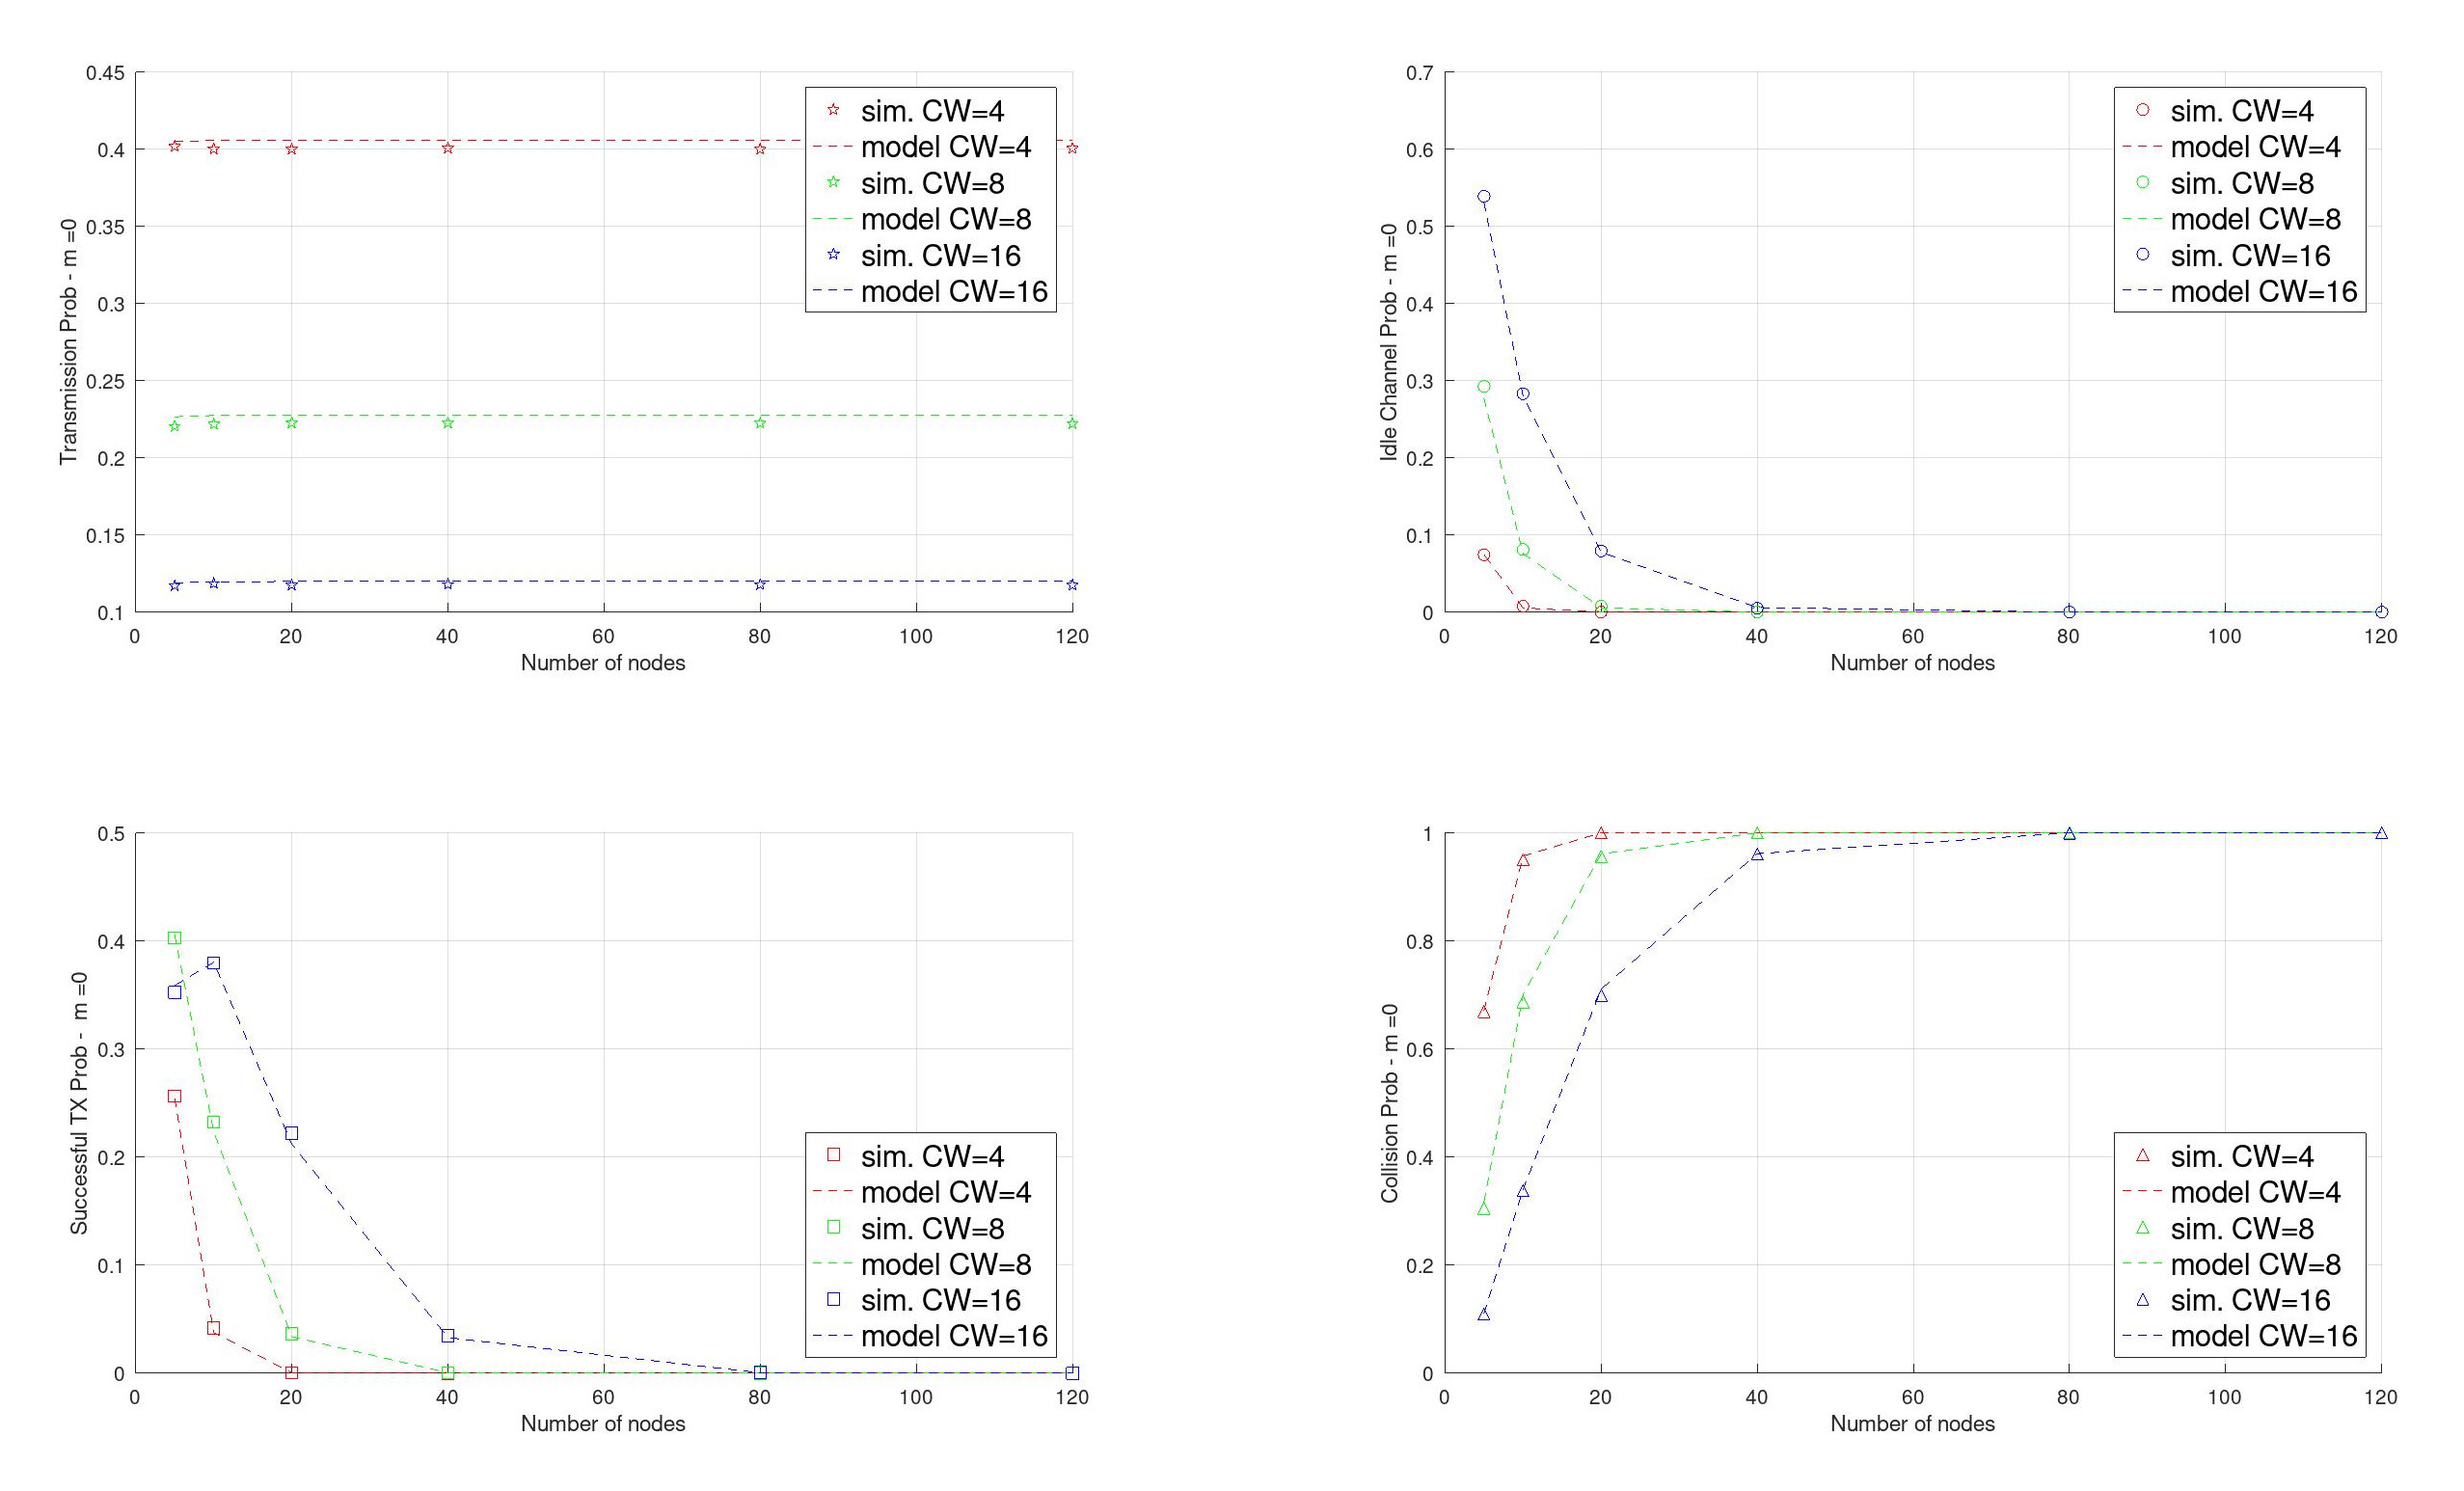
\includegraphics[scale=.18]{Images/objetivo1m0.jpeg}
    \caption{Resultados para \textit{m} = 0}
    \label{fig:objetivo1m0}
\end{figure}
\vspace{\baselineskip}

\vspace{\baselineskip}
\begin{figure}[h]
    \centering
    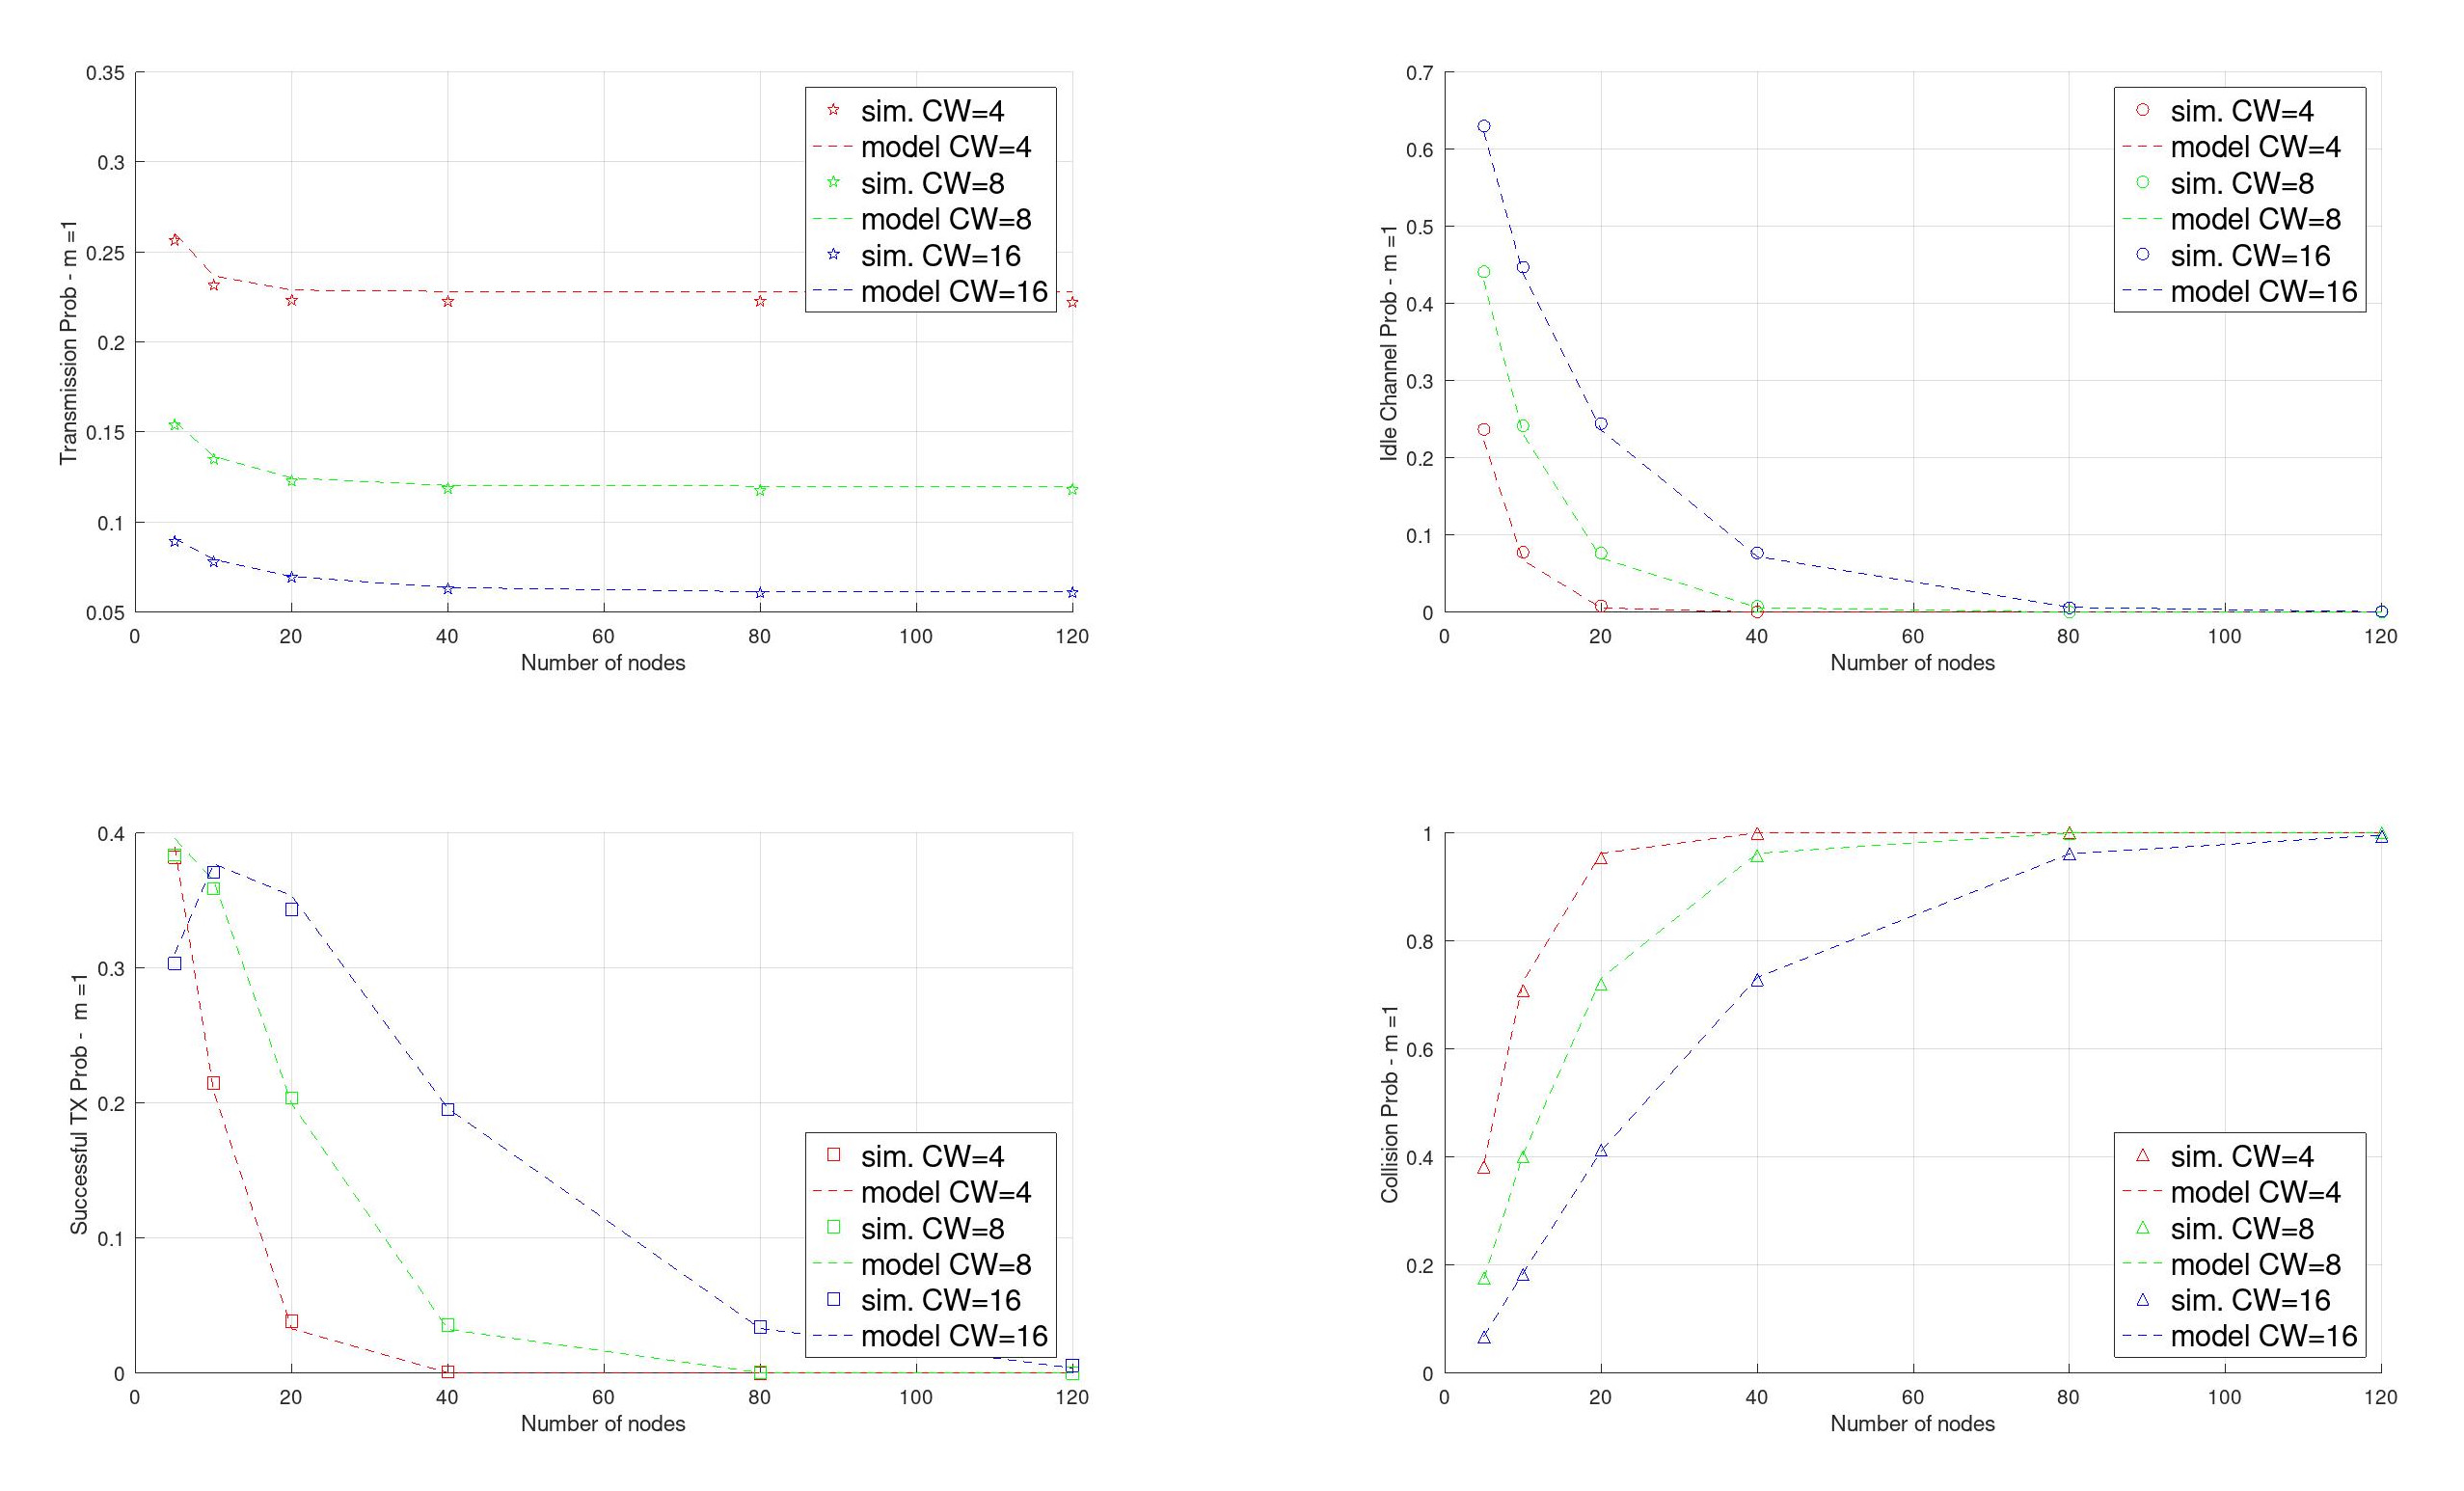
\includegraphics[scale=.18]{Images/objetivo1m1.jpeg}
    \caption{Resultados para \textit{m} = 1}
    \label{fig:objetivo1m1}
\end{figure}
\vspace{\baselineskip}

Nas Figuras \ref{fig:objetivo1m0} e \ref{fig:objetivo1m1} podemos ver os resultados para
\textit{m} = 0 e \textit{m} = 1.
Os resultados do modelo estão de acordo com os da simulação. Com \textit{m} = 0,
os nós nunca irão retransmitir um pacote, logo irão ter a sua janela de transmissão
entre 0 e \textit{CW}. Assim: a probabilidade de transmissão é sempre a mesma.
Com uma janela de transmissão tão baixa, os nós vão estar sempre a tentar transmitir,
e para um alto número de nós irão existir demasiadas colisões, e muito poucas
(ou nenhumas) transmissões bem-sucedidas.
Para \textit{m} = 1, já existe uma retransmissão em caso de colisão, e a janela de transmissão
máxima será $\textit{CW}^2$. Para poucos nós a probabilidade de transmissão bem-sucedida é boa
(por volta dos 30\%), mas para casos com 40 ou mais nós essa probabilidade já é afetada, e a
probabilidade de colisãp começa a ser alta.

\vspace{\baselineskip}
\begin{figure}[h]
    \centering
    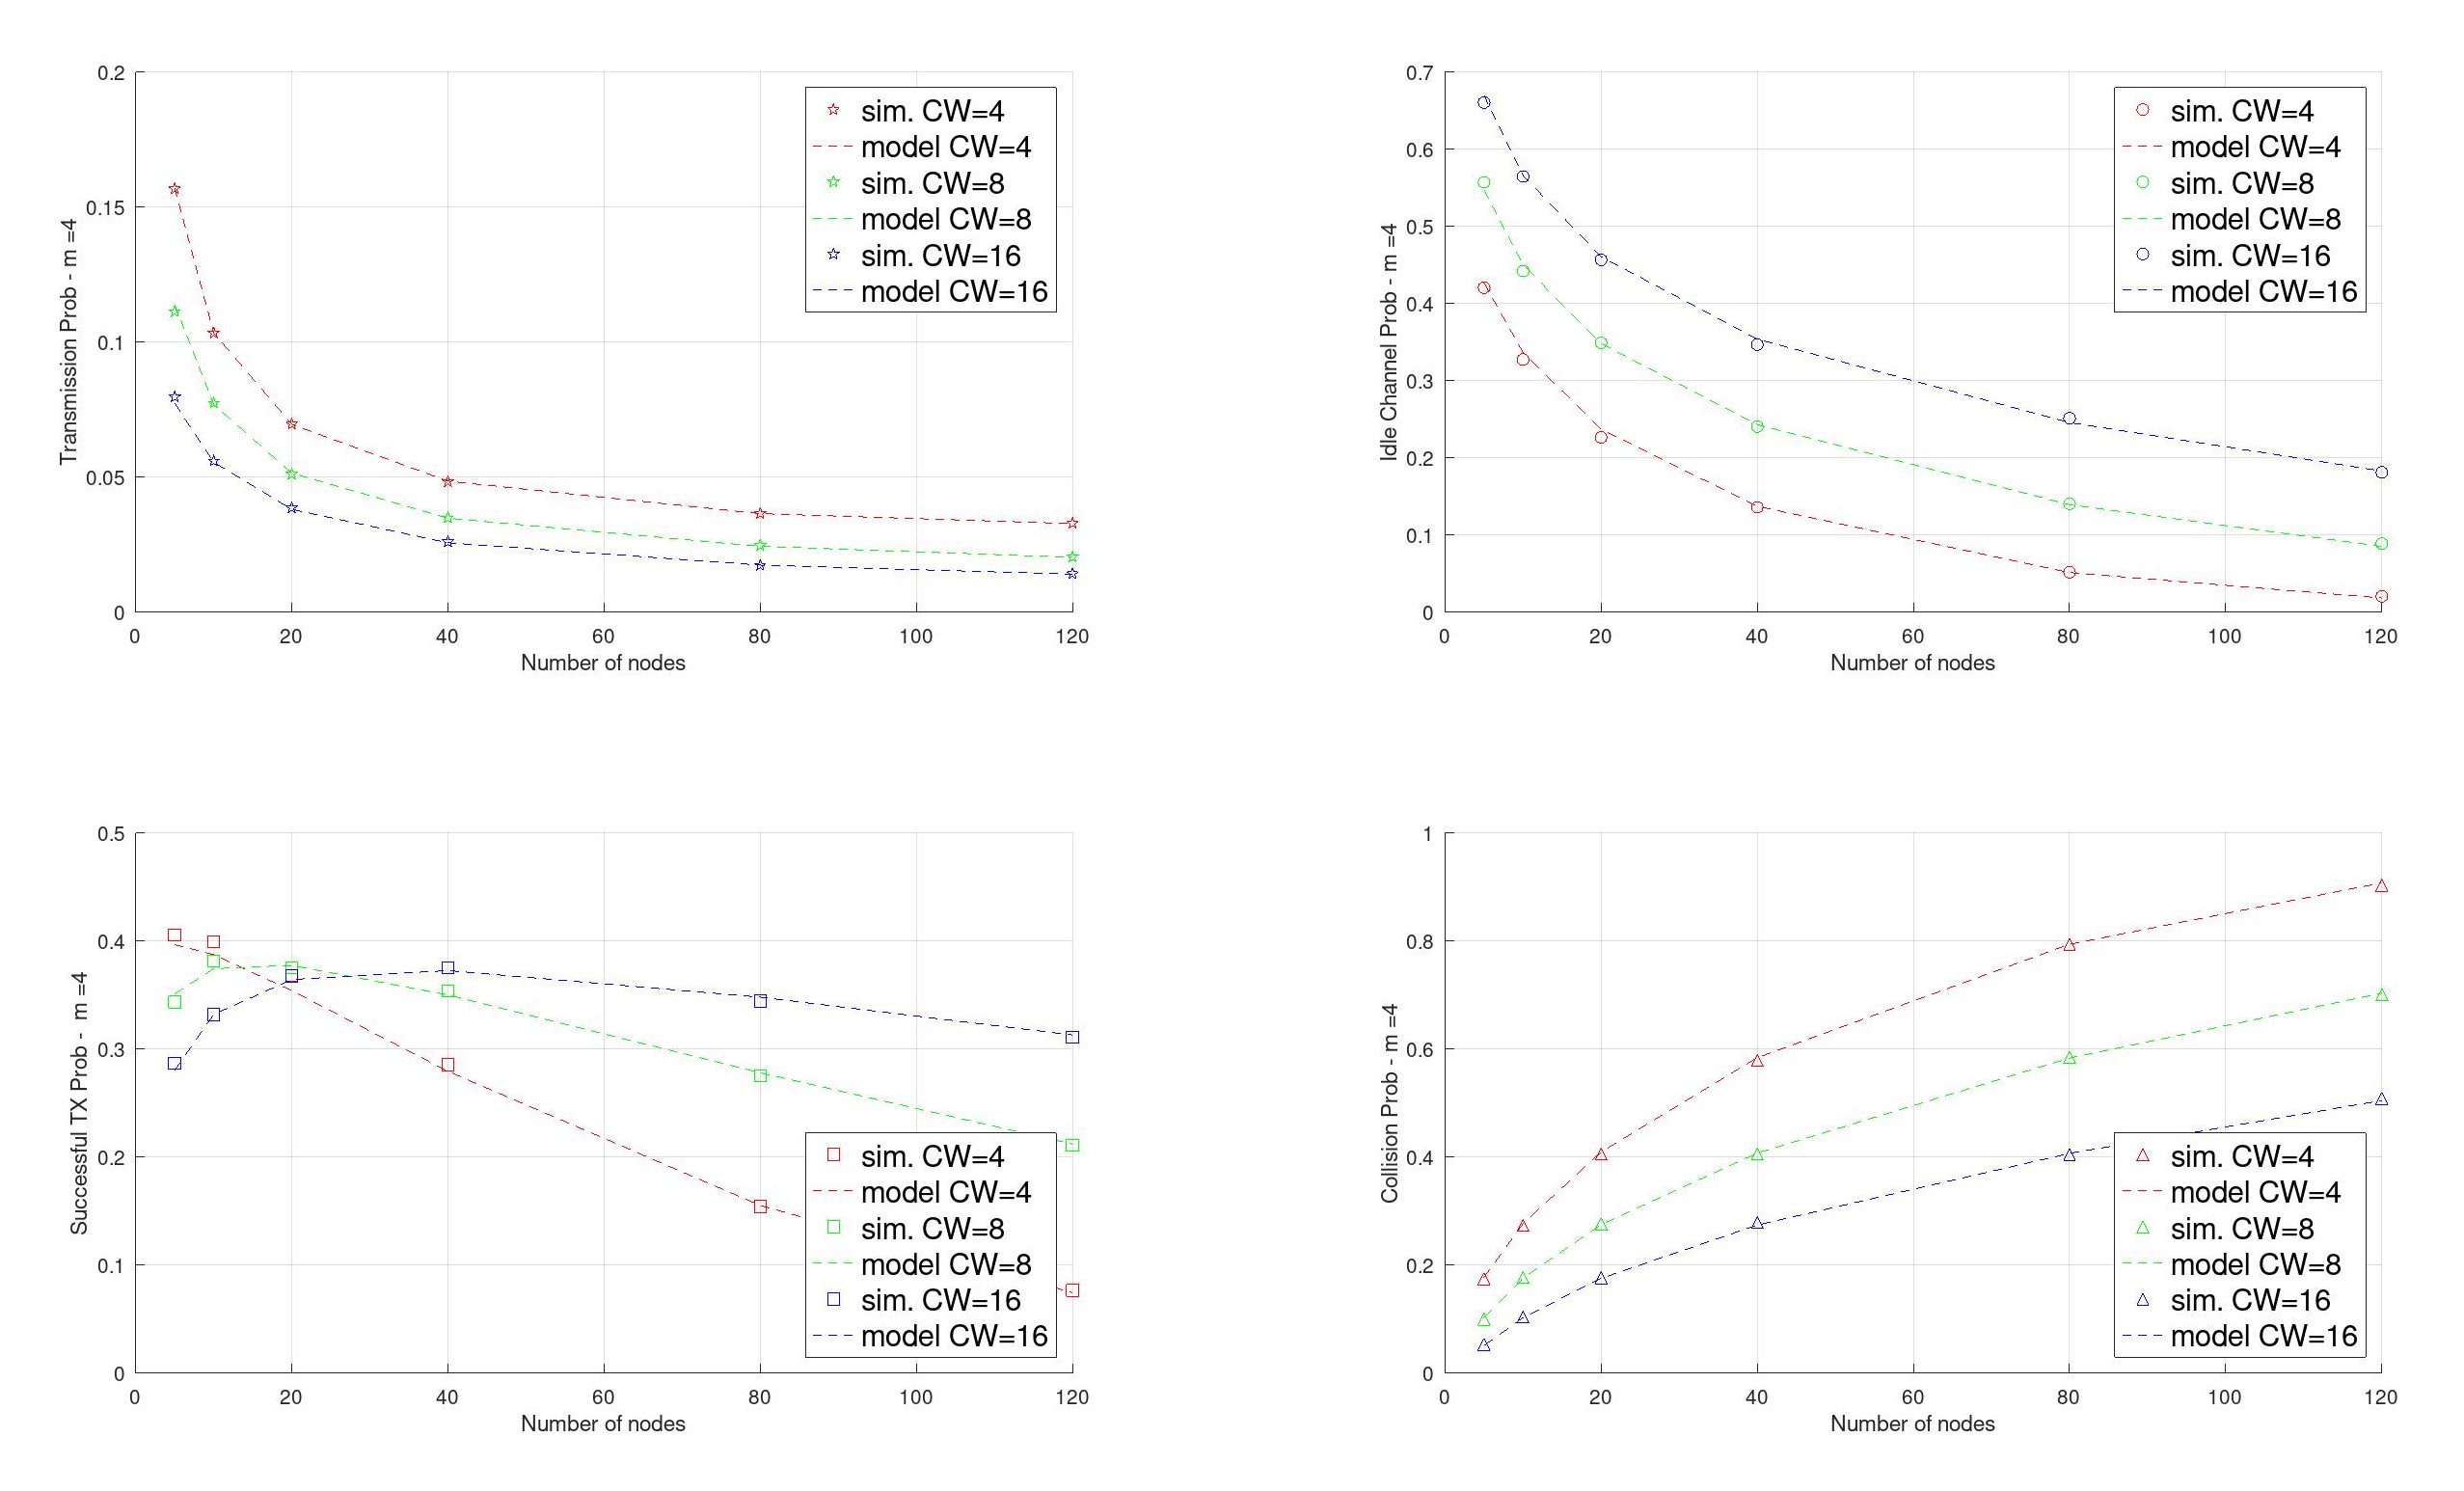
\includegraphics[scale=.18]{Images/objetivo1m4.jpeg}
    \caption{Resultados para \textit{m} = 4}
    \label{fig:objetivo1m4}
\end{figure}
\vspace{\baselineskip}

Na Figura \ref{fig:objetivo1m4} podemos ver os resultados para \textit{m} = 4.
Os resultados do modelo estão de acordo com os da simulação. Aqui podemos observar como
o aumento de \textit{m} afeta positivamente a probabilidade de transmissão
bem-sucedida, diminuindo a taxa de colisão. A probabilidade
de sucesso começa alta, por volta dos 35\%, mas baixa bastante para um elevado número
de nós e para uma janela de transmissão máxima \textit{CW} baixa. Para valores de \textit{CW}
altos, a probabilidade de sucesso mantém-se acima dos 30\% para até 120 nós.
Assim, podemos também concluir que valores de \textit{CW} altos conseguem lidar
bastante melhor com números de nós muito altos.


\vspace{\baselineskip}
\begin{figure}[h]
    \centering
    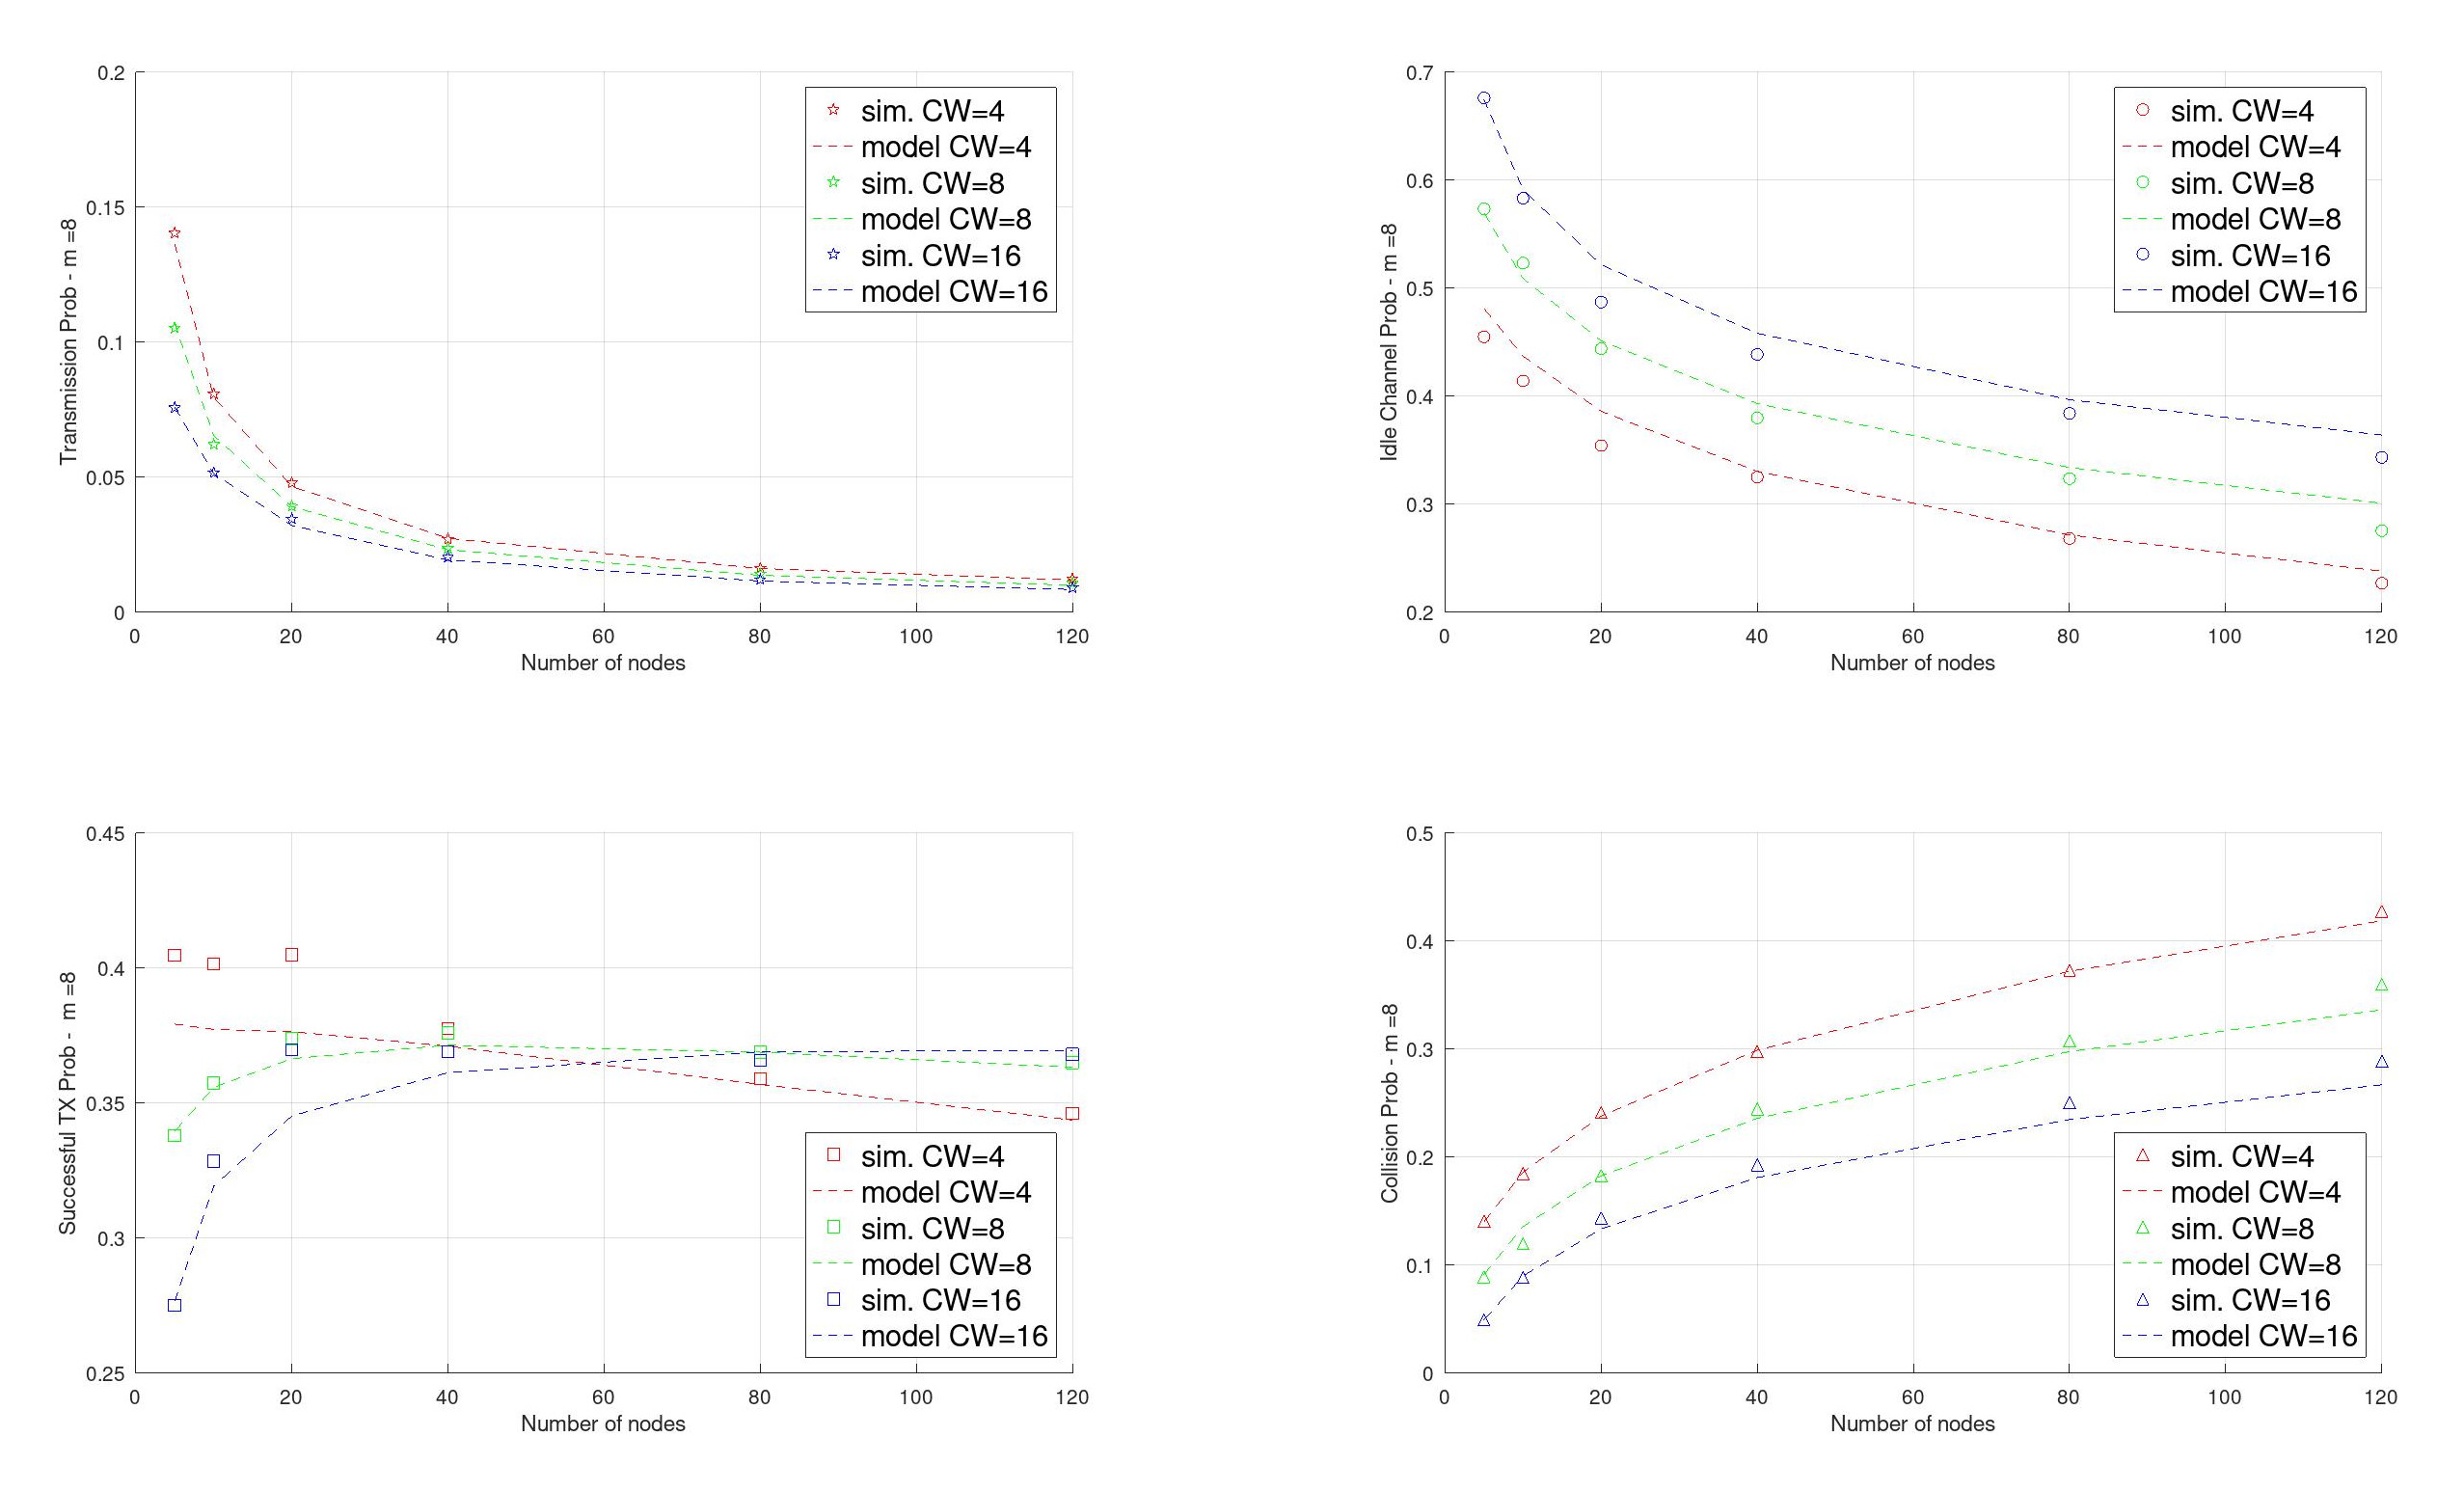
\includegraphics[scale=.18]{Images/objetivo1m8.jpeg}
    \caption{Resultados para \textit{m} = 8}
    \label{fig:objetivo1m8}
\end{figure}
\vspace{\baselineskip}

\vspace{\baselineskip}
\begin{figure}[h]
    \centering
    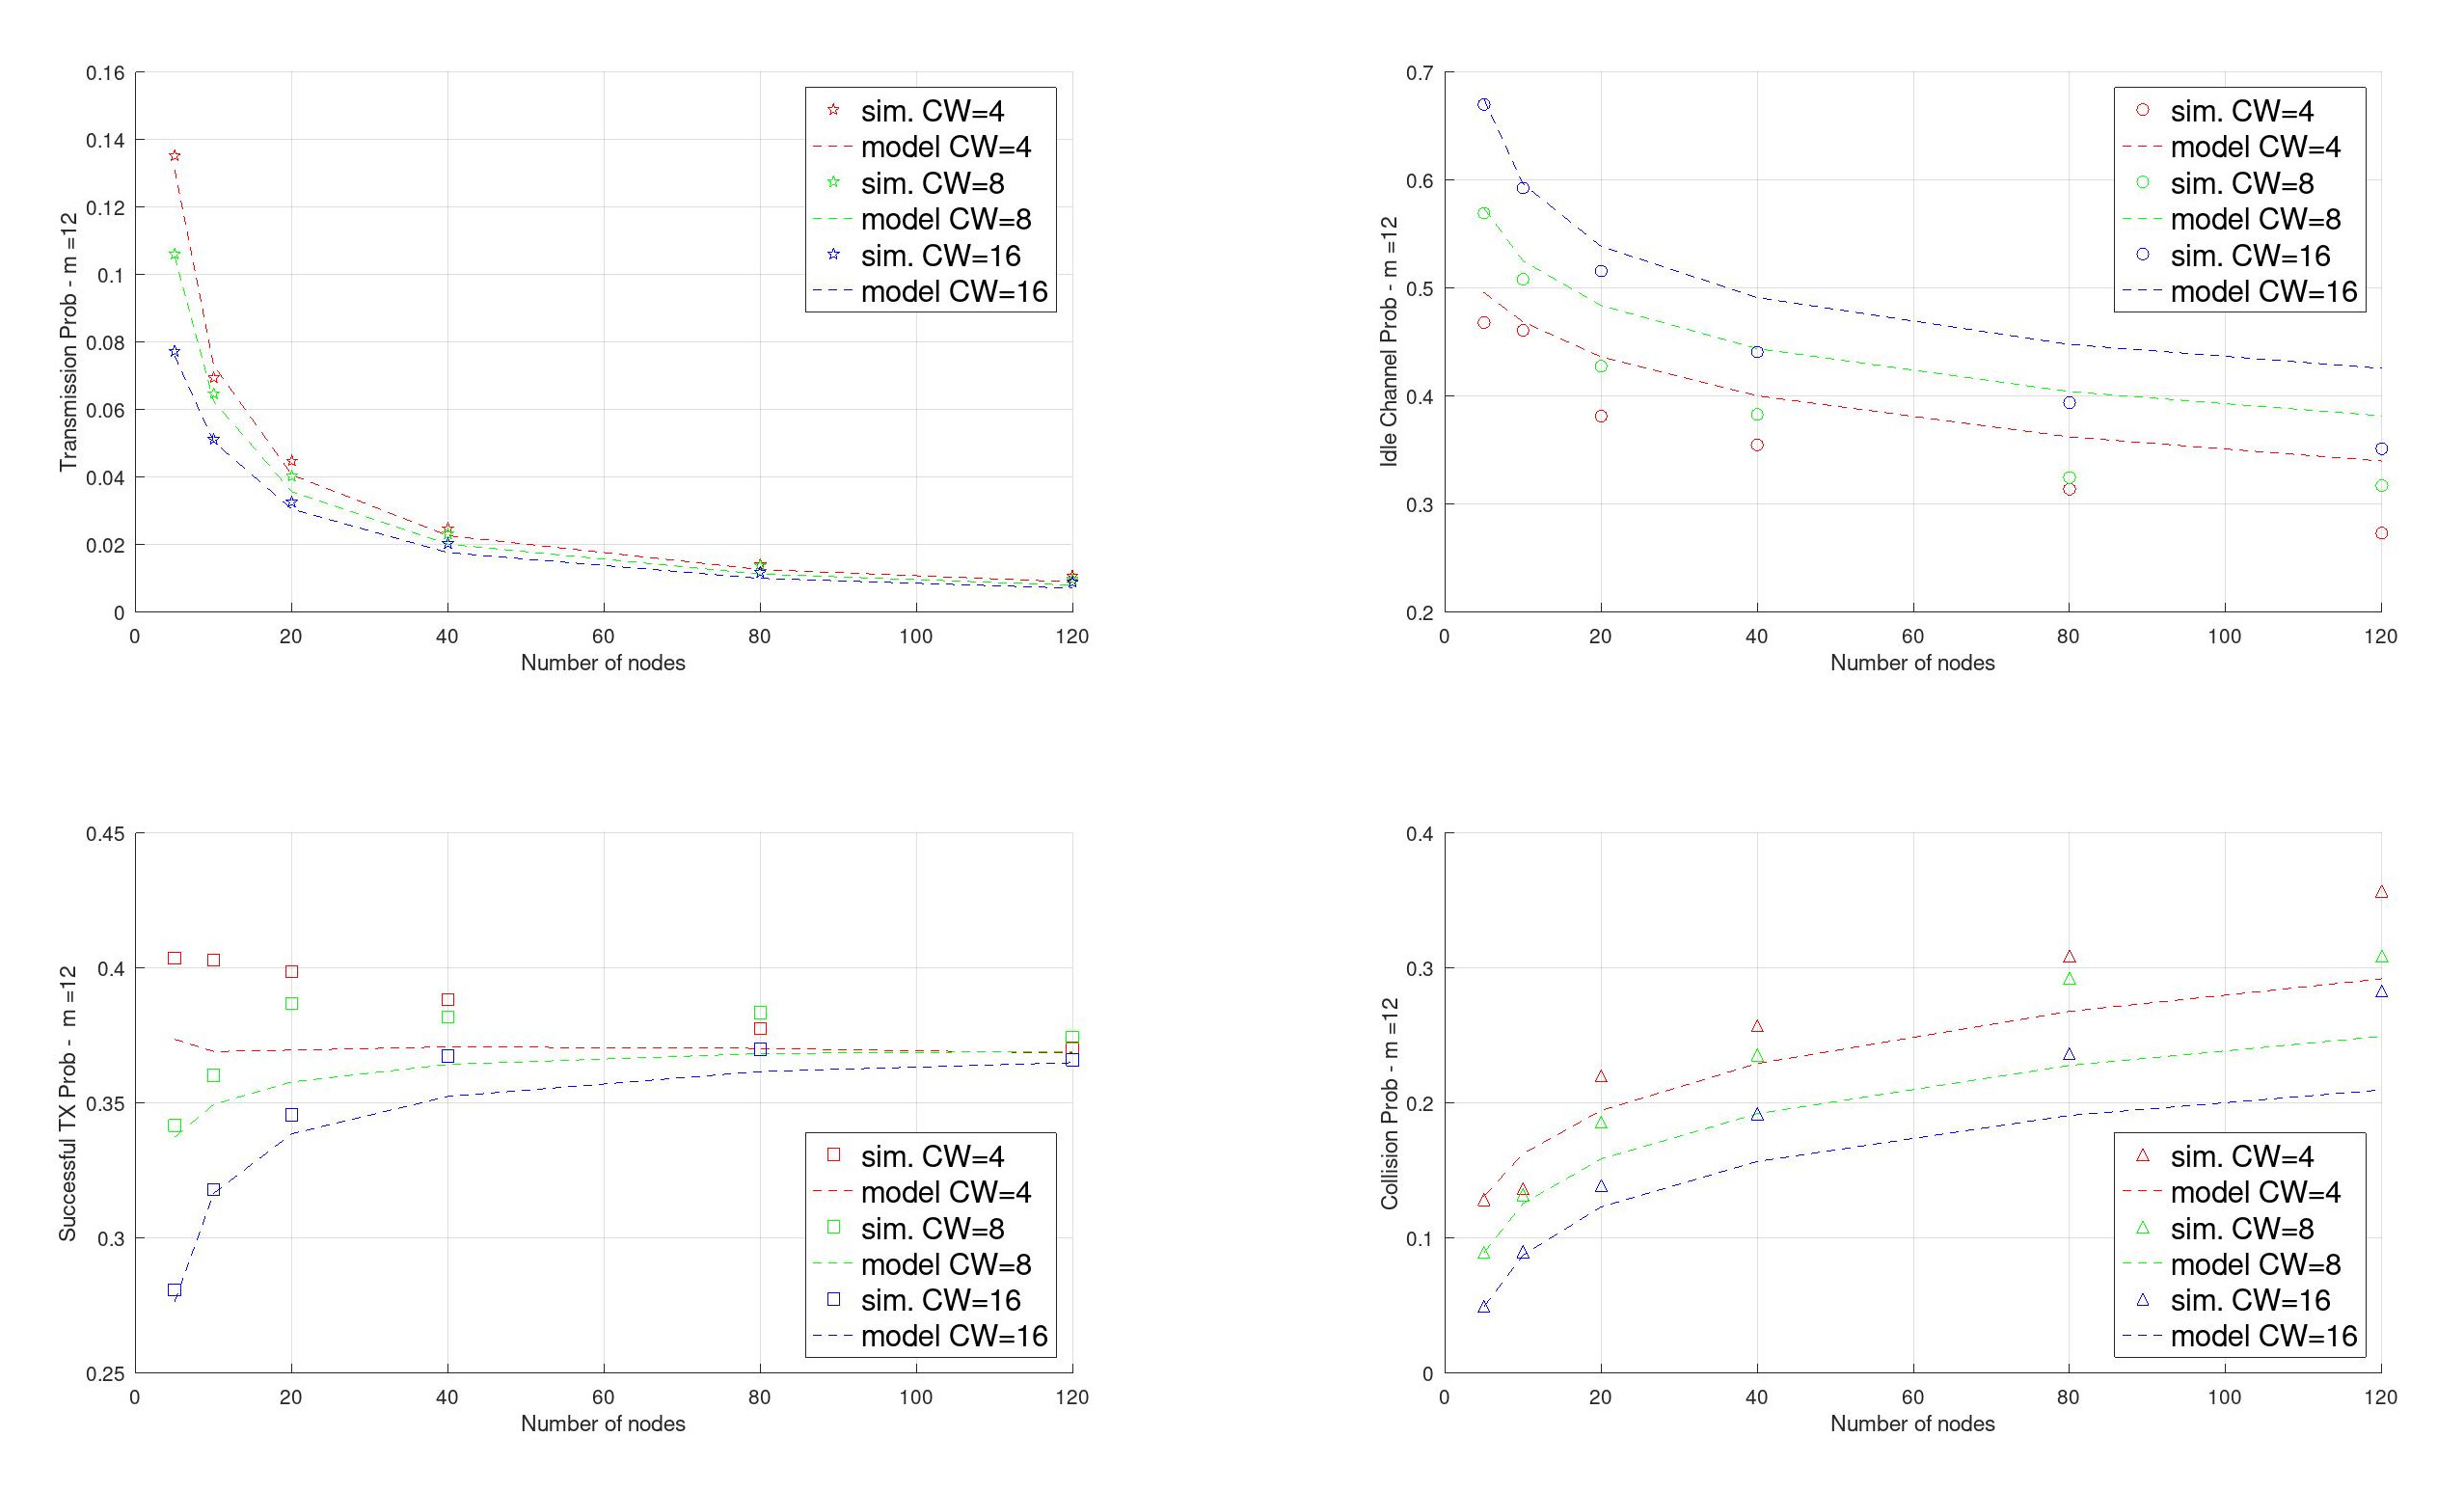
\includegraphics[scale=.18]{Images/objetivo1m12.jpeg}
    \caption{Resultados para \textit{m} = 12}
    \label{fig:objetivo1m12}
\end{figure}
\vspace{\baselineskip}

Nas Figuras \ref{fig:objetivo1m8} e \ref{fig:objetivo1m12} podemos ver os resultados para
\textit{m} = 8 e \textit{m} = 12. Aqui, os resultados do modelo já começam a desviar-se
da simulação, especialmente nas probabilidade de colisão e de canal livre
no caso de \textit{m} = 12.
No que toca à simulação, os valores entre os 2 gráficos são bastante idênticos.
Podemos, mais uma vez, observar que valores de \textit{CW} baixos funcionam melhor
para pequenos números de nós. Para bastantes nós, a probabilidade de transmissão
bem-sucedida converge para os 40\%, o melhor valor de todos os casos. Os valores da
probabilidade de colisão são significativamente inferiores comparados a valores
obtidos para \textit{m} = 8 mais baixos.

\vspace{\baselineskip}

Todos estes resultados foram obtidos através dos ficheiros em anexo
\textit{main.m}, \textit{simulation.m} e \textit{model.m}.